\documentclass[11pt]{article}
\usepackage[margin=0.75in]{geometry}
\usepackage{amsmath,amssymb}
\usepackage{xcolor}
\usepackage{tikz}
\usepackage[most]{tcolorbox}
\usepackage{enumitem}
\usepackage{titlesec}
\usepackage{fancyhdr}

\definecolor{ink}{HTML}{1F3A5F}
\definecolor{key}{HTML}{8A1C1C}
\definecolor{soft}{HTML}{EEF3F8}
\definecolor{warm}{HTML}{FBF3E6}

\setlength{\parindent}{0pt}
\setlength{\parskip}{4pt}
\setlist{itemsep=1pt,topsep=2pt}
\titleformat{\section}{\large\bfseries\color{ink}}{\thesection.}{0.5em}{}
\titleformat{\subsection}{\normalsize\bfseries\color{ink}}{}{0em}{}
\titlespacing*{\section}{0pt}{10pt}{4pt}
\titlespacing*{\subsection}{0pt}{6pt}{2pt}

\newcommand{\E}{\mathrm{E}}

\newtcolorbox{bigidea}{colback=soft,colframe=ink,boxrule=0.6pt,arc=2pt,left=5pt,right=5pt,top=3pt,bottom=3pt,
  title={\bfseries\small Big idea},fonttitle=\small}
\newtcolorbox{trap}{colback=warm,colframe=key,boxrule=0.6pt,arc=2pt,left=5pt,right=5pt,top=3pt,bottom=3pt,
  title={\bfseries\small Traps / what graders look for},fonttitle=\small}
\newtcolorbox{answer}{colback=white,colframe=ink,boxrule=0.6pt,arc=2pt,left=6pt,right=6pt,top=4pt,bottom=4pt,
  title={\bfseries\small Model answer},fonttitle=\small,breakable}

\pagestyle{fancy}
\fancyhf{}
\renewcommand{\headrulewidth}{0pt}
\fancyfoot[C]{\small\thepage}

% Shared TikZ figures for the ECON 5040 midterm study guide and sample midterm.
% Each \fig... macro draws one self-contained tikzpicture.

% 1. Intertemporal budget line: R is minus the slope
\newcommand{\figIntertemporal}{%
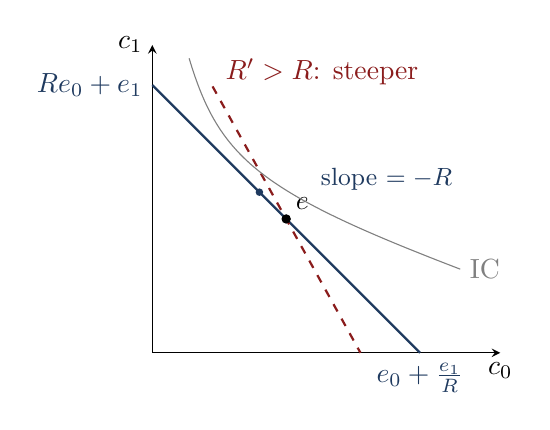
\begin{tikzpicture}[scale=0.85,>=stealth]
  \draw[->] (0,0) -- (5.2,0) node[below] {$c_0$};
  \draw[->] (0,0) -- (0,4.6) node[left] {$c_1$};
  % endowment e = (2,2); budget with R = 1 (slope -1) and R' > R (slope -1.8)
  \draw[thick,ink] (0,4) -- (4,0) node[below] {$e_0+\tfrac{e_1}{R}$};
  \node[left,ink] at (0,4) {$Re_0+e_1$};
  \draw[thick,key,dashed] (0.9,3.98) -- (3.11,0);
  \node[key,right] at (0.95,4.2) {$R'>R$: steeper};
  \fill (2,2) circle (2pt) node[above right] {$e$};
  % indifference curve tangent to the original line at (1.6,2.4)
  \draw[gray] (0.55,4.4) .. controls (1.0,2.9) and (1.6,2.4) .. (4.6,1.25);
  \fill[ink] (1.6,2.4) circle (1.6pt);
  \node[gray,right] at (4.6,1.25) {IC};
  \node[ink] at (3.5,2.6) {\small slope $=-R$};
\end{tikzpicture}}

% 2. Concave utility, expected utility, certainty equivalent
\newcommand{\figCE}{%
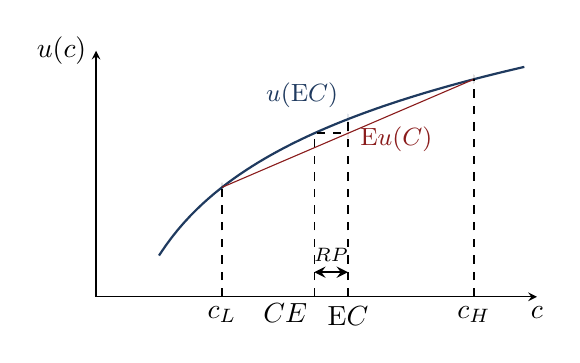
\begin{tikzpicture}[xscale=0.032,yscale=1.25,>=stealth]
  \draw[->] (0,2.8) -- (175,2.8) node[below] {$c$};
  \draw[->] (0,2.8) -- (0,5.3) node[left] {$u(c)$};
  \draw[thick,ink,domain=25:170,samples=60] plot (\x,{ln(\x)});
  \draw[key] (50,{ln(50)}) -- (150,{ln(150)});
  \fill (50,{ln(50)}) circle (1.4pt); \fill (150,{ln(150)}) circle (1.4pt);
  % E[C]=100, E[u]=0.5(ln50+ln150)=4.4637, CE=86.6, u(100)=4.6052
  \fill[key] (100,4.4637) circle (1.6pt);
  \fill[ink] (100,4.6052) circle (1.6pt);
  \draw[dashed] (100,2.8) node[below] {$\E C$} -- (100,4.6052);
  \draw[dashed] (86.6,2.8) node[below left=-1pt] {$CE$} -- (86.6,4.4637) -- (100,4.4637);
  \draw[dashed] (50,2.8) node[below] {$c_L$} -- (50,{ln(50)});
  \draw[dashed] (150,2.8) node[below] {$c_H$} -- (150,{ln(150)});
  \node[ink,above left] at (100,4.62) {\small $u(\E C)$};
  \node[key,right] at (101,4.40) {\small $\E u(C)$};
  \draw[<->,thick] (86.6,3.05) -- node[above] {\scriptsize $RP$} (100,3.05);
\end{tikzpicture}}

% 3. Two-state Markov chain
\newcommand{\figMarkov}{%
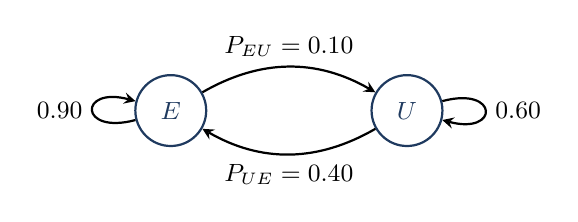
\begin{tikzpicture}[>=stealth,node distance=3cm,every node/.style={font=\small}]
  \node[circle,draw,thick,ink,minimum size=9mm] (E) {$E$};
  \node[circle,draw,thick,ink,minimum size=9mm,right of=E] (U) {$U$};
  \draw[->,thick] (E) to[bend left] node[above] {$P_{EU}=0.10$} (U);
  \draw[->,thick] (U) to[bend left] node[below] {$P_{UE}=0.40$} (E);
  \draw[->,thick] (E) to[loop left] node[left] {$0.90$} (E);
  \draw[->,thick] (U) to[loop right] node[right] {$0.60$} (U);
\end{tikzpicture}}

% 4. Bellman decomposition / timing
\newcommand{\figBellman}{%
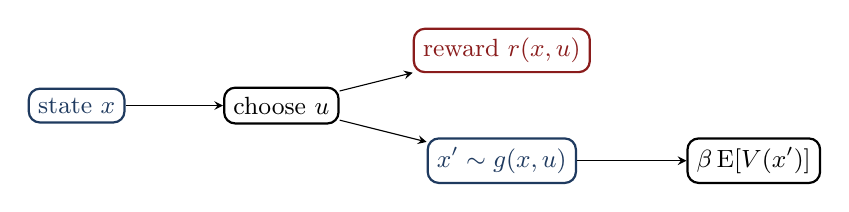
\begin{tikzpicture}[>=stealth,every node/.style={font=\small}]
  \node[draw,rounded corners,ink,thick] (x) at (0,0) {state $x$};
  \node[draw,rounded corners,thick] (u) at (2.6,0) {choose $u$};
  \node[draw,rounded corners,key,thick] (r) at (5.4,0.7) {reward $r(x,u)$};
  \node[draw,rounded corners,ink,thick] (xp) at (5.4,-0.7) {$x'\sim g(x,u)$};
  \node[draw,rounded corners,thick] (v) at (8.6,-0.7) {$\beta\,\E[V(x')]$};
  \draw[->] (x) -- (u); \draw[->] (u) -- (r); \draw[->] (u) -- (xp); \draw[->] (xp) -- (v);
\end{tikzpicture}}

% 5. Solow: sf(k) vs delta k, with a rise in s
\newcommand{\figSolow}{%
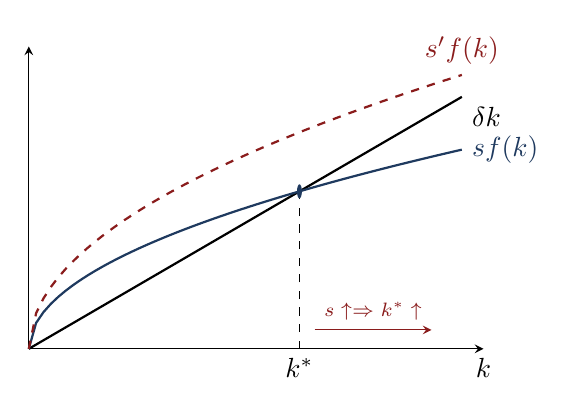
\begin{tikzpicture}[xscale=0.55,yscale=1.6,>=stealth]
  \draw[->] (0,0) -- (10.5,0) node[below] {$k$};
  \draw[->] (0,0) -- (0,2.4);
  \draw[thick] (0,0) -- (10,2) node[below right] {$\delta k$};
  \draw[thick,ink,domain=0:10,samples=60] plot (\x,{0.4*sqrt(\x)*1.25}) node[right] {$sf(k)$};
  \draw[thick,key,dashed,domain=0:10,samples=60] plot (\x,{0.55*sqrt(\x)*1.25}) node[above] {$s'f(k)$};
  % k* where 0.5 sqrt k = 0.2 k -> k = 6.25 ; k*' where 0.6875 sqrt k = 0.2k -> k = 11.8 (off-axis) so use 0.55*1.25=0.6875
  \draw[dashed] (6.25,0) node[below] {$k^*$} -- (6.25,1.25);
  \fill[ink] (6.25,1.25) circle (1.6pt);
  \draw[->,key] (6.6,0.15) -- (9.3,0.15) node[midway,above] {\scriptsize $s\uparrow\Rightarrow k^*\uparrow$};
  
\end{tikzpicture}}

% 6. Level effect vs growth effect
\newcommand{\figLevelGrowth}{%
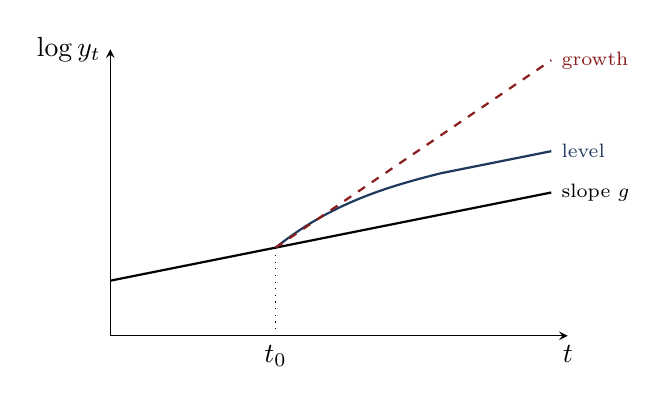
\begin{tikzpicture}[xscale=0.7,yscale=0.7,>=stealth]
  \draw[->] (0,0) -- (8.3,0) node[below] {$t$};
  \draw[->] (0,0) -- (0,5.2) node[left] {$\log y_t$};
  \draw[thick] (0,1) -- (8,2.6) node[right] {\scriptsize slope $g$};
  \draw[thick,ink] (3,1.6) .. controls (4,2.4) and (5,2.7) .. (6,2.95) -- (8,3.35) node[right] {\scriptsize level};
  \draw[thick,key,dashed] (3,1.6) -- (8,5.0) node[right] {\scriptsize growth};
  \draw[dotted] (3,0) node[below] {$t_0$} -- (3,1.6);
\end{tikzpicture}}

% 7. Convex marginal utility -> precautionary saving
\newcommand{\figPrecaution}{%
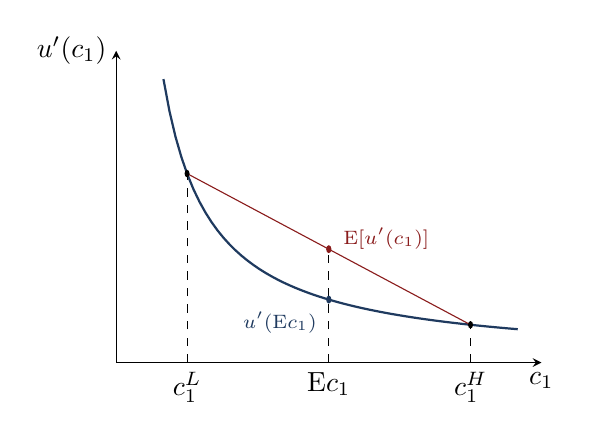
\begin{tikzpicture}[xscale=0.6,yscale=0.9,>=stealth]
  \draw[->] (0,0) -- (9,0) node[below] {$c_1$};
  \draw[->] (0,0) -- (0,4.4) node[left] {$u'(c_1)$};
  \draw[thick,ink,domain=1:8.5,samples=60] plot (\x,{4/\x});
  \draw[key] (1.5,2.667) -- (7.5,0.533);
  \fill (1.5,2.667) circle (1.5pt); \fill (7.5,0.533) circle (1.5pt);
  \draw[dashed] (1.5,0) node[below] {$c_1^L$} -- (1.5,2.667);
  \draw[dashed] (7.5,0) node[below] {$c_1^H$} -- (7.5,0.533);
  \draw[dashed] (4.5,0) node[below] {$\E c_1$} -- (4.5,1.6);
  \fill[key] (4.5,1.6) circle (1.6pt); \fill[ink] (4.5,0.889) circle (1.6pt);
  \node[key,right] at (4.6,1.75) {\scriptsize $\E[u'(c_1)]$};
  \node[ink,below left] at (4.45,0.85) {\scriptsize $u'(\E c_1)$};
\end{tikzpicture}}

% 8. McCall reservation wage
\newcommand{\figMcCall}{%
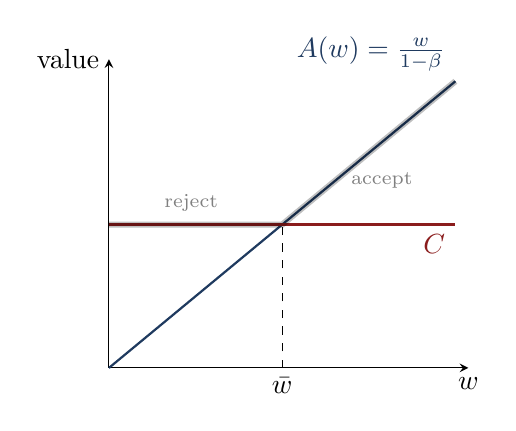
\begin{tikzpicture}[xscale=0.55,yscale=0.7,>=stealth]
  \draw[->] (0,0) -- (8.3,0) node[below] {$w$};
  \draw[->] (0,0) -- (0,5.6) node[left] {value};
  \draw[thick,ink] (0,0) -- (8,5.2) node[above left] {$A(w)=\frac{w}{1-\beta}$};
  \draw[thick,key] (0,2.6) -- (8,2.6) node[below left] {$C$};
  \draw[dashed] (4,0) node[below] {$\bar w$} -- (4,2.6);
  \draw[line width=2.2pt,opacity=0.25] (0,2.6) -- (4,2.6) -- (8,5.2);
  \node[gray] at (1.9,3.0) {\scriptsize reject};
  \node[gray] at (6.3,3.4) {\scriptsize accept};
\end{tikzpicture}}


\newtcolorbox{resp}{colback=white,colframe=ink,boxrule=0.6pt,arc=2pt,left=6pt,right=6pt,top=4pt,bottom=4pt,
  title={\bfseries\small Sample response (write this)},fonttitle=\small,breakable}
\newtcolorbox{intu}{colback=soft,colframe=ink,boxrule=0.4pt,arc=2pt,left=6pt,right=6pt,top=3pt,bottom=3pt,
  title={\bfseries\small Intuition (why it's true)},fonttitle=\small,breakable}

\usepackage{needspace}
\newcounter{qn}
\newcommand{\question}[1]{\par\needspace{16\baselineskip}\refstepcounter{qn}\medskip
{\bfseries\color{ink}\large \theqn.\ #1}\par\smallskip}

\begin{document}
\newgeometry{margin=0.65in}

\begin{center}
{\LARGE\bfseries\color{ink} ECON 5040 Midterm, In Words}\\[3pt]
{\small What to actually write for each of the 10 topics, in plain English, with the intuition underneath so you understand it rather than memorize it.\\
Formulas are kept to the one or two you'd naturally mention. Fisher grades whether you can explain the idea, not whether you can derive it.}
\end{center}

\begin{tcolorbox}[colback=warm,colframe=key,boxrule=0.6pt,arc=2pt,title={\bfseries\small The recipe for every answer},fonttitle=\small]
\small (1) Name the idea in one plain sentence. (2) Say what it means for a person's decision (the trade-off). (3) Say what happens when something changes, and \emph{why}. (4) If there's a classic picture, sketch it and label it.
\end{tcolorbox}

%------------------------------------------------------------
\question{Inter-temporal prices}
\textit{How does the real interest rate set the price of consumption today versus the future? What substitution incentive does a higher rate create?}

\begin{resp}
Consumption today and consumption next year are really two different goods, and the real interest rate is the price that trades one for the other. If I give up one unit of consumption today and save it, I get $1+r$ units next year, so the interest rate tells me how expensive it is to consume now instead of later. When the interest rate rises, consuming today gets more expensive and consuming in the future gets cheaper, because every unit I save now turns into more future consumption. That gives me an incentive to substitute away from consumption today and toward saving for the future; this is the substitution effect, and it always points toward saving more.
\end{resp}
\begin{intu}
Think of it as a store with two shelves, ``now'' and ``later.'' The interest rate is the exchange rate between the shelves. A higher rate is like a sale on the ``later'' shelf, so you buy more of it. The only caveat (mention it if you have room): someone who is already a saver also becomes richer when rates rise, and that income effect might lead them to consume more today. That's why the \emph{total} effect on saving is ambiguous, even though the substitution effect alone is not.
\end{intu}

%------------------------------------------------------------
\question{Choice under uncertainty}
\textit{Explain expected utility and risk aversion. Compute and interpret the certainty equivalent of a 50/50 gamble between 50 and 150 with log utility.}

\begin{resp}
\begin{minipage}[t]{0.6\textwidth}\vspace{0pt}
Under expected utility, people value a risky prospect by averaging the \emph{utility} of each outcome rather than averaging the outcomes themselves. If the utility function is concave, extra consumption adds less and less happiness, so losing 50 hurts more than gaining 50 helps, and the person is risk averse. The certainty equivalent is the sure amount the person likes exactly as much as the gamble; with log utility the 50/150 gamble has a certainty equivalent of about 86.60, even though its average is 100. The gap of about 13.40 is the risk premium, what the person would pay to get rid of the risk, and the more curved the utility function, the bigger that gap.
\end{minipage}\hfill
\begin{minipage}[t]{0.36\textwidth}\vspace{0pt}\centering
\scalebox{0.8}{\figCE}
\end{minipage}
\end{resp}
\begin{intu}
Curvature is the whole story. A straight-line utility (risk neutral) values the gamble at its average, 100. A bent utility drags the value down because the bad outcome lands where utility is steep (each dollar matters a lot) and the good outcome lands where it is flat (each dollar matters little). How to get 86.60: average the logs, then undo the log; with log utility that's just the geometric mean, $\sqrt{50\times150}$.
\end{intu}

%------------------------------------------------------------
\question{Markov processes}
\textit{What is the Markov property? How do you interpret an element $P_{ij}$ and a whole row of a transition matrix?}

\begin{resp}
A process is Markov if knowing today's state is enough to forecast tomorrow: once you know where you are now, the rest of the history gives no extra information about where you'll go next. The past can still matter, but only because it got you to today's state. In a transition matrix, the element $P_{ij}$ is the probability of moving to state $j$ tomorrow given that you're in state $i$ today; for example, the unemployed-to-employed entry is the job-finding rate. A whole row is the complete set of possibilities for tomorrow starting from one state today, so its entries are all nonnegative and add up to one.
\end{resp}
\begin{intu}
Rows are ``where I am,'' columns are ``where I might go.'' Reading across a row answers: ``If I'm unemployed today, what are my odds tomorrow?'' The Markov assumption is what makes dynamic models manageable: you only have to track the current state, not a person's whole life story. A nice extra line: even when everyone keeps moving between states, the \emph{share} of people in each state can settle down to a steady (stationary) distribution.
\end{intu}

%------------------------------------------------------------
\question{Introduction to dynamic programming}
\textit{Explain the Bellman equation. Identify the state, choice, current payoff, and next-period state in a dynamic problem.}

\begin{resp}
The Bellman equation breaks a long-horizon problem into two pieces: what I get today, and how good my situation will be tomorrow, discounted because the future matters a bit less. So instead of planning my whole life at once, I make one choice today, knowing I'll keep acting optimally from then on. The \emph{state} is everything I need to know right now to decide (like my capital or wealth), the \emph{choice} is what I control (like how much to save), the \emph{current payoff} is today's utility from that choice, and the \emph{next-period state} is where the choice leaves me tomorrow. In the growth model, for example, the state is today's capital, the choice is how much capital to carry into tomorrow, the payoff is the utility of whatever output I consume, and tomorrow's state is the capital I kept.
\end{resp}
\begin{intu}
Today's choice matters twice: it changes what I enjoy now \emph{and} where I start tomorrow. The value function packages ``all of tomorrow and beyond'' into one number, so the hard infinite problem becomes ``today's reward $+$ discounted value of where I land.'' The catch is that the value function shows up on both sides, so you have to solve for it (that's what Topic 6 is about). To find the state, ask: ``What would I need to write on a sticky note to make today's decision?''
\end{intu}

%------------------------------------------------------------
\question{Value functions and policy functions}
\textit{Distinguish the two. What information does each give, and how does the policy relate to the Bellman equation?}

\begin{resp}
The value function tells you \emph{how good} it is to be in a given state, assuming you behave optimally from now on; it's a measure of lifetime welfare. The policy function tells you \emph{what to do} in each state, such as how much to save or whether to accept a job, so it's a complete contingency plan. The policy is simply the choice that maximizes the right-hand side of the Bellman equation: today's reward plus the discounted value of tomorrow. Once you know the value function you can read off the best action in every state, and once you follow that policy forever you get back the value function.
\end{resp}
\begin{intu}
Value $=$ ``how good is my position?'' (a score). Policy $=$ ``what's my move?'' (a rule). In an uncertain world the answer can't be a fixed list of actions, because you don't know which states will happen, so it has to be a rule for every state. Example: in job search the value function says how good each wage offer is, while the policy is just ``accept if the offer is above the reservation wage.''
\end{intu}

%------------------------------------------------------------
\question{Howard's method versus value function iteration}
\textit{Explain the logic of each and why Howard can be much faster.}

\begin{resp}
Value function iteration starts with a guess of the value function and keeps plugging it into the Bellman equation, so each round adds one more period of future rewards, until the guess stops changing. Howard's method instead starts with a guess of the \emph{policy}, works out exactly how valuable it would be to follow that policy forever (policy evaluation), and then checks whether switching actions in any state would do better (policy improvement). It repeats these two steps until the policy no longer changes. Howard is usually much faster because each evaluation step jumps straight to the full long-run value of a policy, instead of creeping toward it one period at a time, so it typically settles on the optimal policy after only a few rounds.
\end{resp}
\begin{intu}
VFI is like walking toward the answer in small steps; when people are very patient (discount factor near 1), the steps are tiny and it takes forever. Howard says: ``Pick a plan, figure out exactly how good it is, then fix whatever's wrong with it.'' With the plan fixed there's nothing left to optimize, so evaluating it is just solving a system of equations. There are only so many possible plans and each round improves, so you finish quickly.
\end{intu}

%------------------------------------------------------------
\question{The Solow model}
\textit{How do saving and capital accumulation determine steady-state capital and output? Level effect vs.\ growth effect.}

\begin{resp}
\begin{minipage}[t]{0.6\textwidth}\vspace{0pt}
In the Solow model a fixed share of output is saved and invested, which adds to the capital stock, while some capital wears out each year. Because each extra unit of capital adds less output than the last (diminishing returns), investment eventually only covers the capital that wears out, and the economy settles at a steady state where capital and output per worker stop changing. A higher saving rate moves that steady state up, so the economy ends up permanently \emph{richer}: a level effect. But it does not permanently raise the growth rate: growth speeds up only during the transition, and in the long run growth per worker comes only from technological progress.
\end{minipage}\hfill
\begin{minipage}[t]{0.36\textwidth}\vspace{0pt}\centering
\scalebox{0.75}{\figSolow}\\[3pt]
\scalebox{0.75}{\figLevelGrowth}
\end{minipage}
\end{resp}
\begin{intu}
Picture a bathtub: investment is the faucet, depreciation is the drain. As capital rises, the faucet (output) grows more and more slowly while the drain grows proportionally, so the water level stops rising. Saving more opens the faucet: the tub fills to a higher level, then stops again. Growth graph in words: the path of log income jumps up to a \emph{parallel} higher line (level effect), and does not swing to a steeper line (growth effect).
\end{intu}

%------------------------------------------------------------
\question{Optimal saving}
\textit{Interpret the Euler equation $u'(c_t)=\beta R\,\E_t[u'(c_{t+1})]$. What does a household do if the two sides aren't equal?}

\begin{resp}
The Euler equation compares two uses of one extra unit of income: eat it today, or save it and eat the proceeds tomorrow. The left side is the extra satisfaction from consuming it now; the right side is the extra satisfaction from saving it, which grows with interest but is discounted because it comes later and is uncertain. At the optimum these are equal, so there is no gain from shifting consumption between today and tomorrow. If consuming today is worth more than saving, the household should consume more and save less; if saving is worth more, it should cut consumption and save more; and these adjustments continue until the two sides balance.
\end{resp}
\begin{intu}
It's a marginal ``is it worth it?'' test, the same MRS-equals-price idea as Topic 1, just repeated every period. Why the adjustment restores balance: eating more today makes the next bite today less valuable (diminishing marginal utility) and leaves less for tomorrow, which makes tomorrow's bite more valuable, so the two sides move toward each other. Exception worth a phrase: if you're up against a borrowing limit, you'd like to consume more today but can't, so the two sides can stay unequal.
\end{intu}

%------------------------------------------------------------
\question{Income fluctuations}
\textit{Why can income uncertainty raise saving even if expected income doesn't change? Why do assets provide self-insurance?}

\begin{resp}
\begin{minipage}[t]{0.6\textwidth}\vspace{0pt}
When future income is uncertain, the bad outcomes are especially painful, because when consumption is low each extra dollar is worth a lot. So a dollar saved today is particularly valuable as protection against a bad draw, and the household saves more than it would if it knew it would get the average income for sure; this is precautionary saving. Assets act as self-insurance because the household can draw them down when income turns out low, moving resources into exactly the future situations where consumption and wealth would otherwise be low. The asset itself pays the same return in every state, but since the household decides how much to spend \emph{after} seeing its income, savings work like a buffer.
\end{minipage}\hfill
\begin{minipage}[t]{0.36\textwidth}\vspace{0pt}\centering
\scalebox{0.8}{\figPrecaution}
\end{minipage}
\end{resp}
\begin{intu}
It's a rainy-day fund. Same average income, but more risk, means more saving, because the downside hurts more than the upside helps. The math reason (one phrase if you want it): marginal utility is convex, so risk raises the \emph{expected} value of an extra future dollar. Distinguish three words: \emph{smoothing} (dislike ups and downs), \emph{self-insurance} (using a buffer of assets), and \emph{precautionary saving} (saving more because of risk itself). Needed context: there's no full insurance market for your income, so you insure yourself.
\end{intu}

%------------------------------------------------------------
\question{Putting it together: job search}
\textit{Why is job search a dynamic problem? Formulate it with a state, choice, transition, and continuation value.}

\begin{resp}
\begin{minipage}[t]{0.6\textwidth}\vspace{0pt}
Job search is dynamic because turning down an offer affects both today and the future: you give up the wage today and collect only unemployment benefits, but you keep the chance of a better offer tomorrow. The \emph{state} is the wage offer you currently hold, the \emph{choice} is to accept or reject it, and the \emph{transition} is that accepting means earning that wage forever while rejecting means drawing a new random offer next period. The \emph{continuation value} is the value of rejecting: benefits today plus the discounted value of searching again optimally tomorrow. Because accepting is worth more the higher the wage, while the continuation value doesn't depend on today's offer, there is a cutoff, the reservation wage, and the worker accepts any offer above it.
\end{minipage}\hfill
\begin{minipage}[t]{0.36\textwidth}\vspace{0pt}\centering
\scalebox{0.8}{\figMcCall}
\end{minipage}
\end{resp}
\begin{intu}
It's a stopping problem: the question isn't ``which wage?'' but ``when do I stop searching?'' Graph in words: the value of accepting is an upward-sloping line in the wage, the value of continuing is a flat line, and they cross at the reservation wage. Comparative statics people like to see: higher unemployment benefits or more patience make waiting more attractive, so the reservation wage rises and search lasts longer.
\end{intu}

\end{document}
